\chapter{Digital Evidence Examination and Analysis}

\section{Filesystem Structure and Organization}

\subsection{Partition Analysis and Key Evidence Locations}
Examination of the imaged drive revealed a dual-partition structure as shown in Figure \ref{fig:partition_structure}:

\begin{itemize}
    \item Unallocated partition 'vol1' (sectors 0-63): Potential location for deleted data
    \item Primary Win95 FAT32 partition 'vol2' (sectors 63-3915584): Main filesystem containing user data
\end{itemize}

\begin{figure}[htbp]
    \centering
    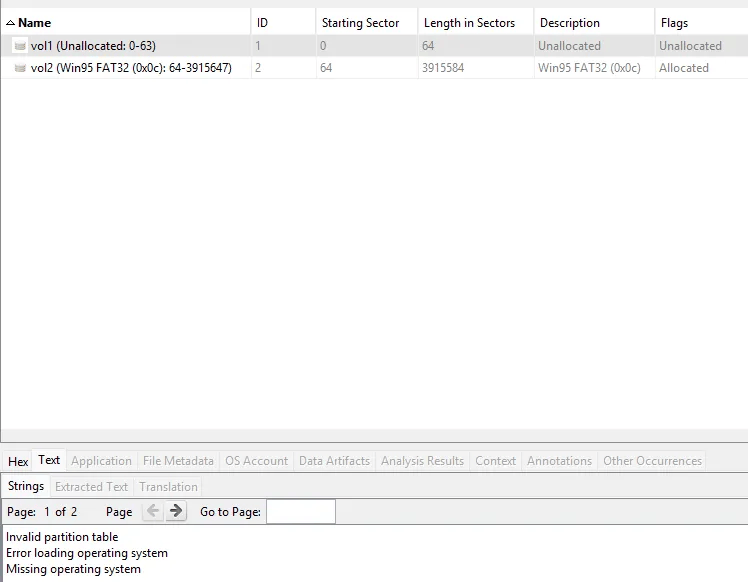
\includegraphics[width=0.8\textwidth]{images/Evidence Examination/Image1.png}
    \caption{Autopsy Partition Analysis View showing the dual-partition structure}
    \label{fig:partition_structure}
\end{figure}

The use of FAT32 rather than NTFS is forensically significant, as FAT32 lacks robust permission structures and encryption capabilities, potentially indicating a preference for portability or cross-platform compatibility over security.

\subsection{File Type Distribution and Suspicious Content}
Analysis of file types across the image (Figure \ref{fig:file_types}) revealed several forensically significant patterns:

\begin{figure}[htbp]
    \centering
    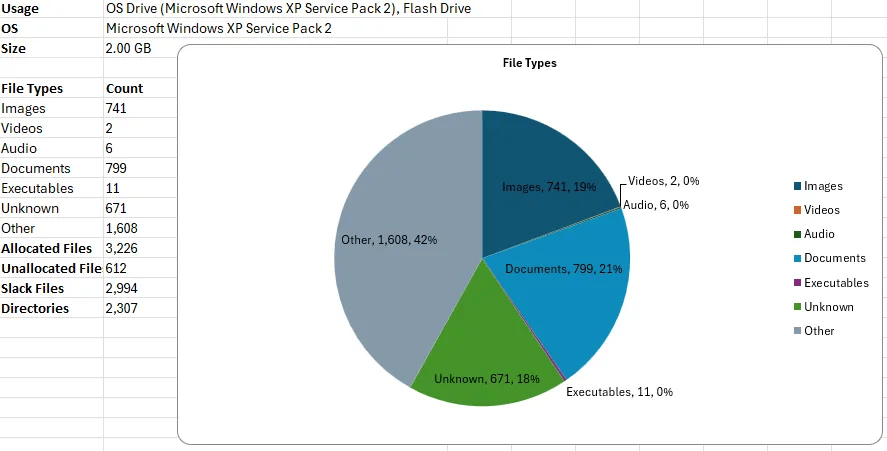
\includegraphics[width=0.8\textwidth]{images/Evidence Examination/Image2.png}
    \caption{File Type Distribution Analysis showing proportions of various file categories}
    \label{fig:file_types}
\end{figure}

\begin{itemize}
    \item 42\% of files classified as "Other": Potential indicator of non-standard file formats or obfuscation
    \item 19\% images (741 files): High priority for steganographic analysis
    \item 18\% Unknown files (671): Possible evidence of deliberate file type manipulation
    \item Total system content: 3,226 allocated and 612 unallocated files
\end{itemize}

The operating system was identified as Microsoft Windows XP Service Pack 2, with the drive containing 2.00 GB of data classified as both an OS Drive and a Flash Drive, suggesting a portable storage medium with system installation.

\subsection{Directory Structure and User Accounts}
As shown in Figure \ref{fig:directory_explorer}, the filesystem contained multiple user profiles with literary-themed naming patterns ("Bilbo Baggins," "Frodo Baggins," "Sam") suggesting deliberate account creation for specific purposes rather than legitimate multi-user functionality.

\begin{figure}[htbp]
    \centering
    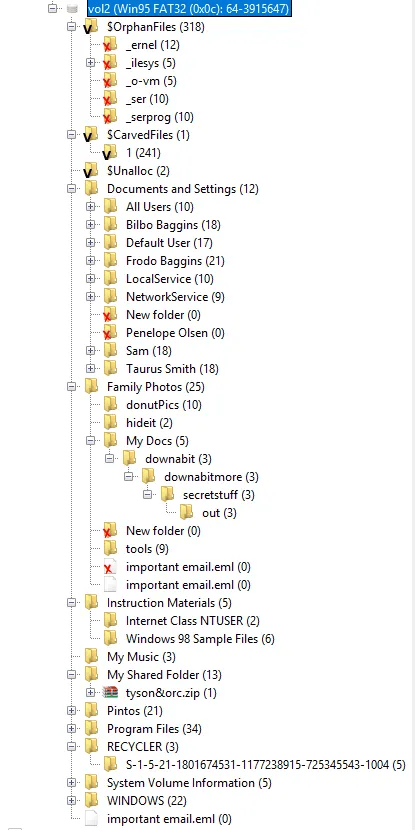
\includegraphics[width=0.6\textwidth]{images/Evidence Examination/Image3.png}
    \caption{Directory Explorer View showing folder structure and suspicious directories}
    \label{fig:directory_explorer}
\end{figure}

Five directories of particular forensic interest were identified in the Taurus Smith directory:

\begin{table}[htbp]
\centering
\begin{tabular}{|p{3cm}|p{6cm}|p{5cm}|}
\hline
\textbf{Directory Name} & \textbf{Forensic Significance} & \textbf{Path} \\
\hline
donutPics (10 files) & Explicitly named directory relevant to alleged recipe theft & /Documents and Settings/Taurus Smith/donutPics \\
\hline
hideit (2 files) & Explicitly suspicious nomenclature suggesting concealment & /Documents and Settings/Taurus Smith/hideit \\
\hline
Family Photos (25 files) & Possible misdirection via innocuous naming & /Documents and Settings/Taurus Smith/Family Photos \\
\hline
My Docs (5 files) & Contains "downabitmore" and "secretstuff" subdirectories & /Documents and Settings/Taurus Smith/My Docs \\
\hline
tools (9 files) & Potential steganography/encryption applications & /Documents and Settings/Taurus Smith/tools \\
\hline
\end{tabular}
\caption{Key Suspicious Directories and their Forensic Significance}
\label{table:suspicious_directories}
\end{table}

Multiple "important email.eml" files were duplicated across the directory structure, suggesting deliberate distribution of communication evidence.

\section{Unallocated Space Recovery and Analysis}

\subsection{Recovered Recipe Evidence}
PhotoRec carving techniques applied to unallocated space recovered a critical file containing proprietary recipe information:

\begin{itemize}
    \item Path: \small{/img\_Taurus Laptop.001/vol\_vol2/\$Unalloc/Unalloc\_8524\_43768320\_1003921408}
    \item Size: 821,198,336 bytes (783 MB)
    \item Content: Hex analysis revealed detailed donut recipe (Figure \ref{fig:hex_view})
\end{itemize}

\begin{figure}[htbp]
    \centering
    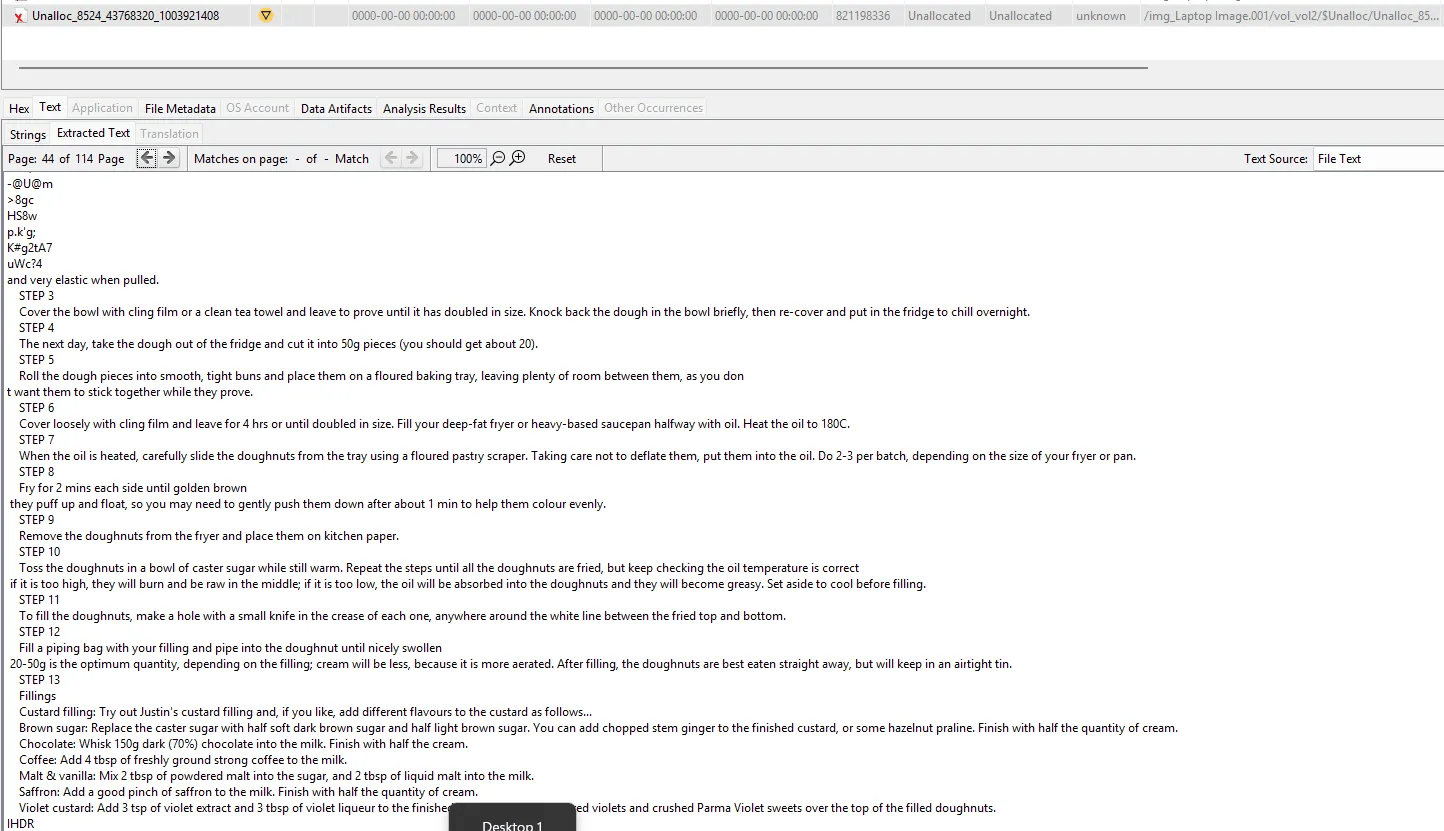
\includegraphics[width=0.95\textwidth]{images/Evidence Examination/Image4.png}
    \caption{Hex View of Recovered Recipe in Unallocated Space showing cooking instructions}
    \label{fig:hex_view}
\end{figure}

The recovered recipe contained professional culinary specifications including precise cooking temperatures (180°C), exact measurements (50g dough portions), and detailed instructions for multiple filling flavors (custard, chocolate, coffee, saffron). The structured, numbered format (STEP 3-13) is consistent with professional documentation rather than casual notes.

\subsection{Travel Evidence}
File carving also recovered a flight plan image (f0066494.png, 636,468 bytes) from unallocated space, shown in Figure \ref{fig:flight_plan}:

\begin{figure}[htbp]
    \centering
    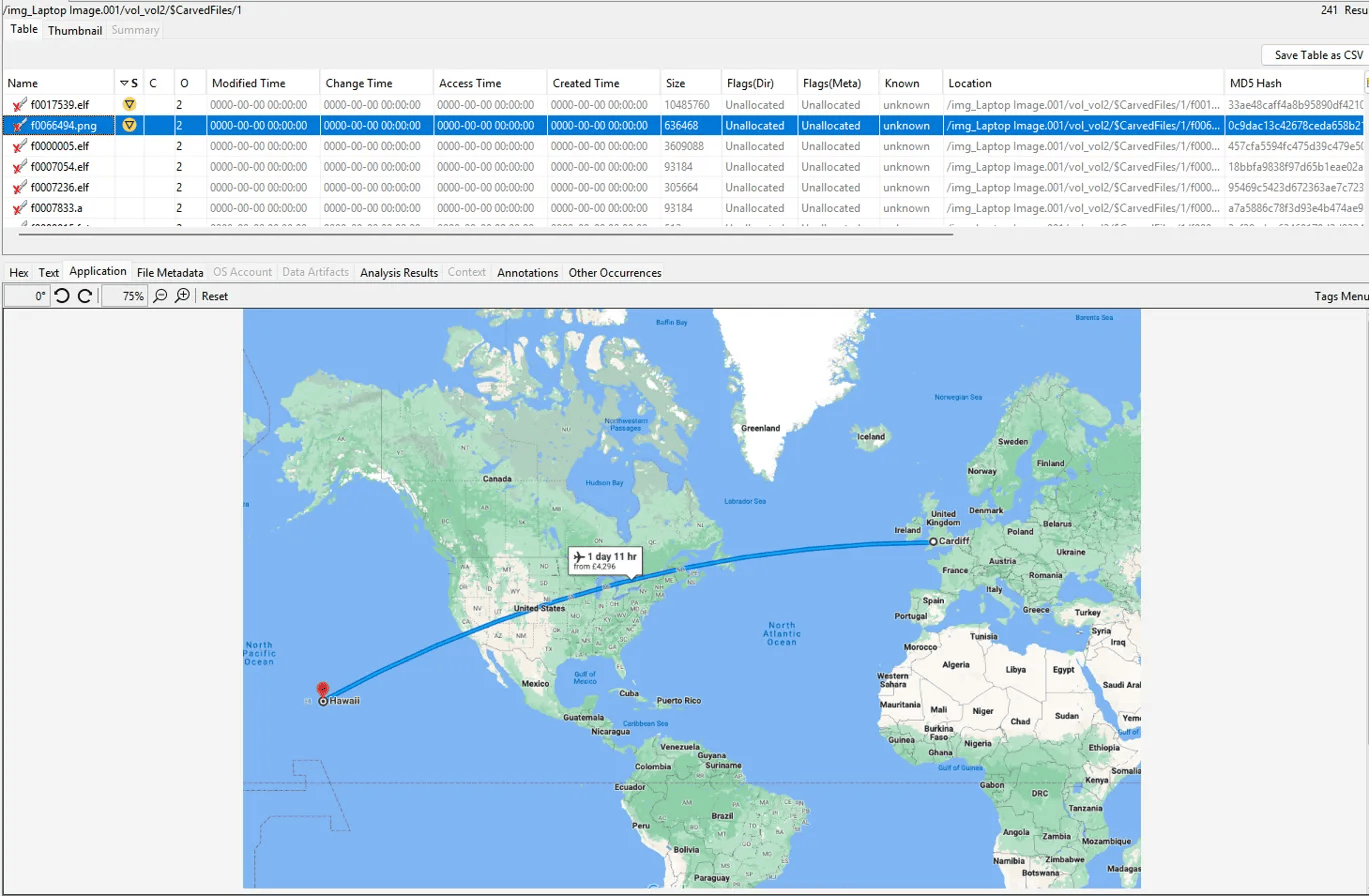
\includegraphics[width=0.95\textwidth]{images/Evidence Examination/Image5.png}
    \caption{Recovered Flight Plan from Cardiff to Hawaii showing travel route and duration}
    \label{fig:flight_plan}
\end{figure}

This image provides direct evidence of planned travel from Cardiff, Wales to Hawaii with a journey time of "1 day 11 hr". All timestamp fields contained null values (0000-00-00 00:00:00), consistent with data recovered from unallocated space. This evidence directly answers investigation question 2 regarding Taurus Smith's travel plans.

\subsection{Steganography Instructions in Recovered Email}
Examination of email artifacts yielded definitive evidence linking to steganography techniques (Figure \ref{fig:email_artifact}):

\begin{figure}[htbp]
    \centering
    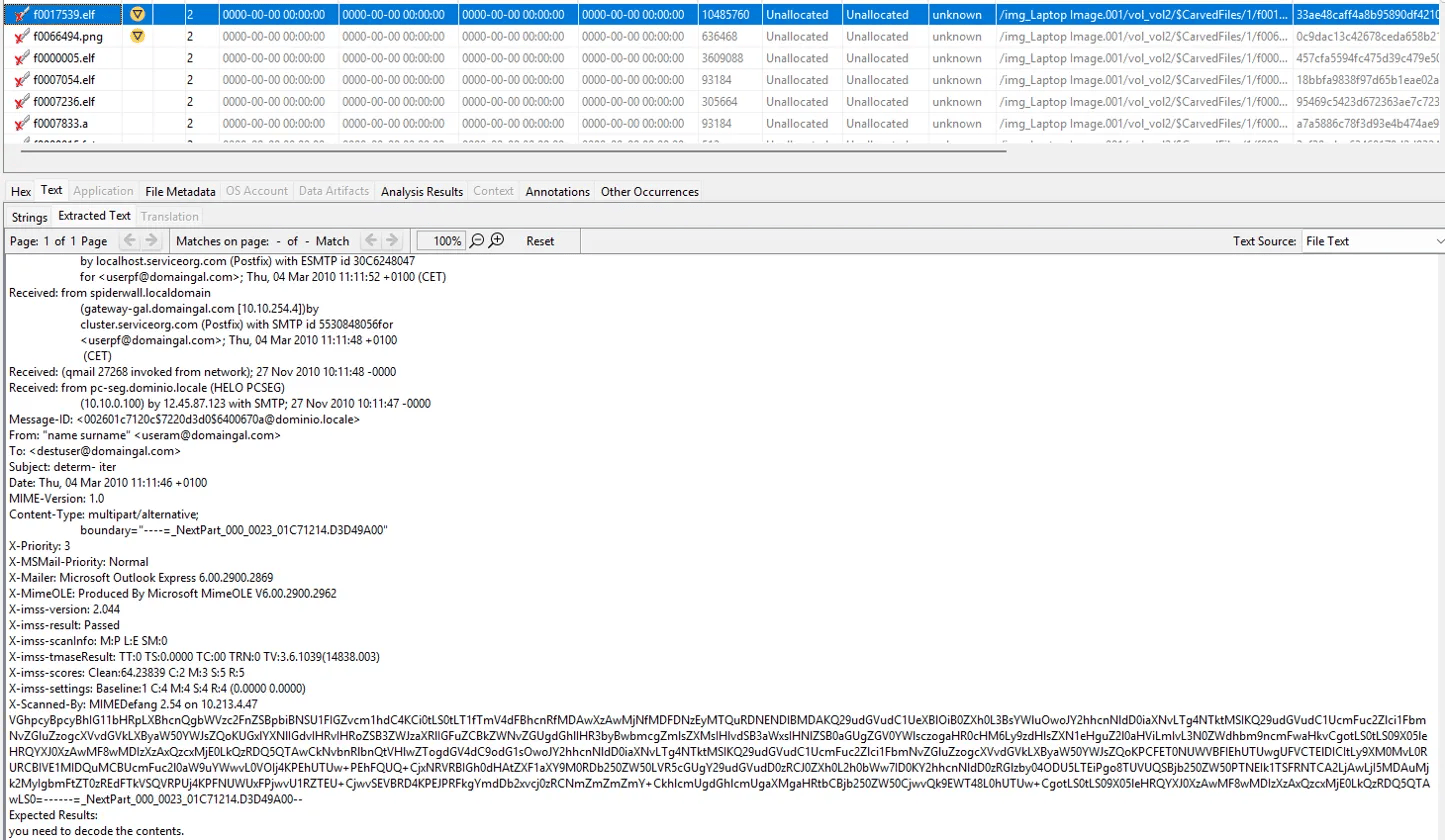
\includegraphics[width=0.95\textwidth]{images/Evidence Examination/Image6.png}
    \caption{Email Artifact Recovery showing Base64-encoded content}
    \label{fig:email_artifact}
\end{figure}

The email recovered from f0017539.elf contained Base64-encoded content that, when decoded, revealed explicit instructions to "go to the website and decode the two png files" with a direct reference to "https://stylesuxx.github.io/steganography/". Key forensic findings include:

\begin{itemize}
    \item Explicit reference to steganographic techniques
    \item Mention of "two png files" matching bean.png and coconuts.png found elsewhere
    \item Identification of the exact steganography tool used
    \item Email header timestamp (March 4, 2010) establishing timeline
\end{itemize}

This email provides direct evidence of intent to conceal and access hidden recipe data using steganography, addressing investigation question 3 regarding recipe concealment techniques.

\section{System Configuration and User Identity Analysis}
Examination of system artifacts revealed configuration details with investigative significance:

\begin{table}[htbp]
\centering
\begin{tabular}{|p{5cm}|p{8.5cm}|}
\hline
\textbf{System Parameter} & \textbf{Forensic Significance} \\
\hline
Operating System & Windows XP Service Pack 2 (outdated, potential security weaknesses) \\
\hline
Computer Name & "FRODO1" (correlates with literary user account naming pattern) \\
\hline
System Owner & "ADXP" (differs from Taurus Smith, suggesting identity obfuscation) \\
\hline
Windows Installation Path & D:\textbackslash{}WINDOWS (non-standard location) \\
\hline
\end{tabular}
\caption{System Configuration Parameters and Investigative Relevance}
\label{table:system_config_significance}
\end{table}

The literary-themed computer name "FRODO1" directly correlates with user account naming patterns, suggesting deliberate persona creation. The divergence between system owner designation ("ADXP") and primary user identity (Taurus Smith) indicates potential identity obfuscation or shared system usage, supporting investigation question 1 regarding additional implicated individuals.